\chapter{Render large list with FlatList}

\section{Video: Rendering large lists using FlatList component}
\subsection{Why FlatList?}
\begin{itemize}
    \item While ScrollView provides a very useful functionality, it does also introduce the issue of slow rendering times for large lists.
    \item FlatList is another approach that can enable faster performance.
    \item Rendreing time with FlatList is not affected by large lists.
    \item For example, using ScrollView with text and images can take a lot of time waiting for rendering because user have to wait for all these images load before they can experience the app.
\end{itemize}

\subsection{FlatList - Lazy rendering}
\begin{itemize}
    \item Instead of rendering the items all at once, FlatList render as the items appear.
    \item Items are only rendered when they are about to appear on the screen and are removed when the user scrolls away from them.
    \item Result in faster rendering and superior performance.
    \item \textbf{Practice Question:} The \texttt{FlatList} component uses lazy rendering of component items. Which of the following are characteristics of lazy rendering? Choose all that apply.
    $\rightarrow$ Items are rendered as the user encounters them in the app, Rendered items are removed when the user scrolls away from them.
\end{itemize}

\subsection{Syntax for FlatList}
\begin{itemize}
    \item Basic use: 
    \begin{lstlisting}[language=Java, numbers=none]
        <FlatList 
            data={items}
            renderItem={renderItem}
        />
    \end{lstlisting}
    \item Props: 
    \begin{lstlisting}[language=Java, numbers=none]
        renderItem({ item, index, separators })
    \end{lstlisting}
    \begin{itemize}
        \item item: single from array.
        \item index: unique index from the data array.
        \item separators: optional, highligh or unhighligh items.
    \end{itemize}
\end{itemize}

\section{Video: Using the FlatList component}
\begin{itemize}
    \item How to use:
    \begin{lstlisting}[language=Java, numbers=none]
        <FlatList
            data={menuItemsToDisplay}
            renderItem={renderItem}
        />
    \end{lstlisting} 
    \item Props:
    \begin{lstlisting}[language=Java, numbers=none]
        // Array of item
        menuItemsToDisplay;

        // Return a HTML tag, custom tag in this case
        const renderItem = ({ item }) => {
            return <Item name={item.name} />
        }
    \end{lstlisting} 

    \item \textbf{Practice Question:} Which properties are required when using the \texttt{FlatList} component? Select all that apply.
    $\rightarrow$ RenderItem, Data
\end{itemize}

\section{Reading: Explore the FlatList Component}
This part is to pratice using FlatList as the same above part's work.

\section{Reading: Exercise: Render a large list using FlatList}
\begin{figure}[H]
    \centering
    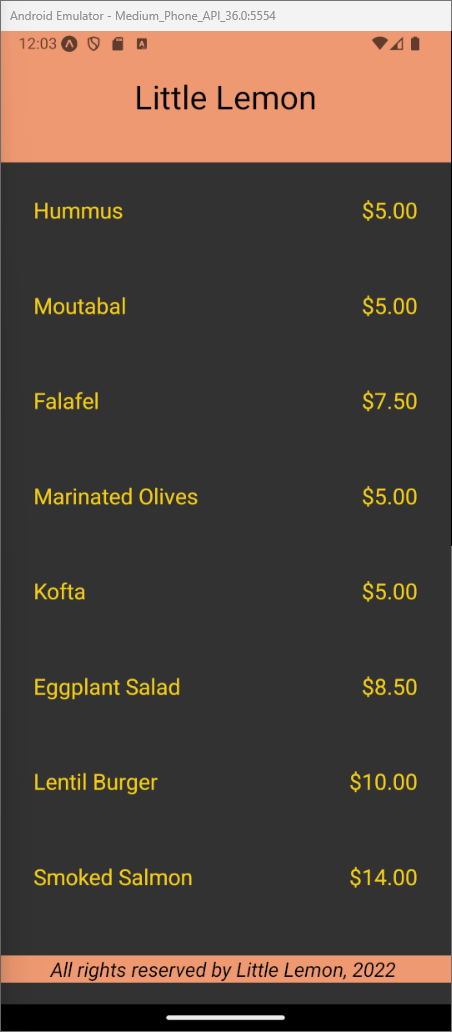
\includegraphics[width=0.2\linewidth]{images/ex1.png}
    \caption{Exercise: Render a large list using FlatList}
\end{figure}

\section{Self review: Render a large list uisng FlatList}
\begin{figure}[H]
    \centering
    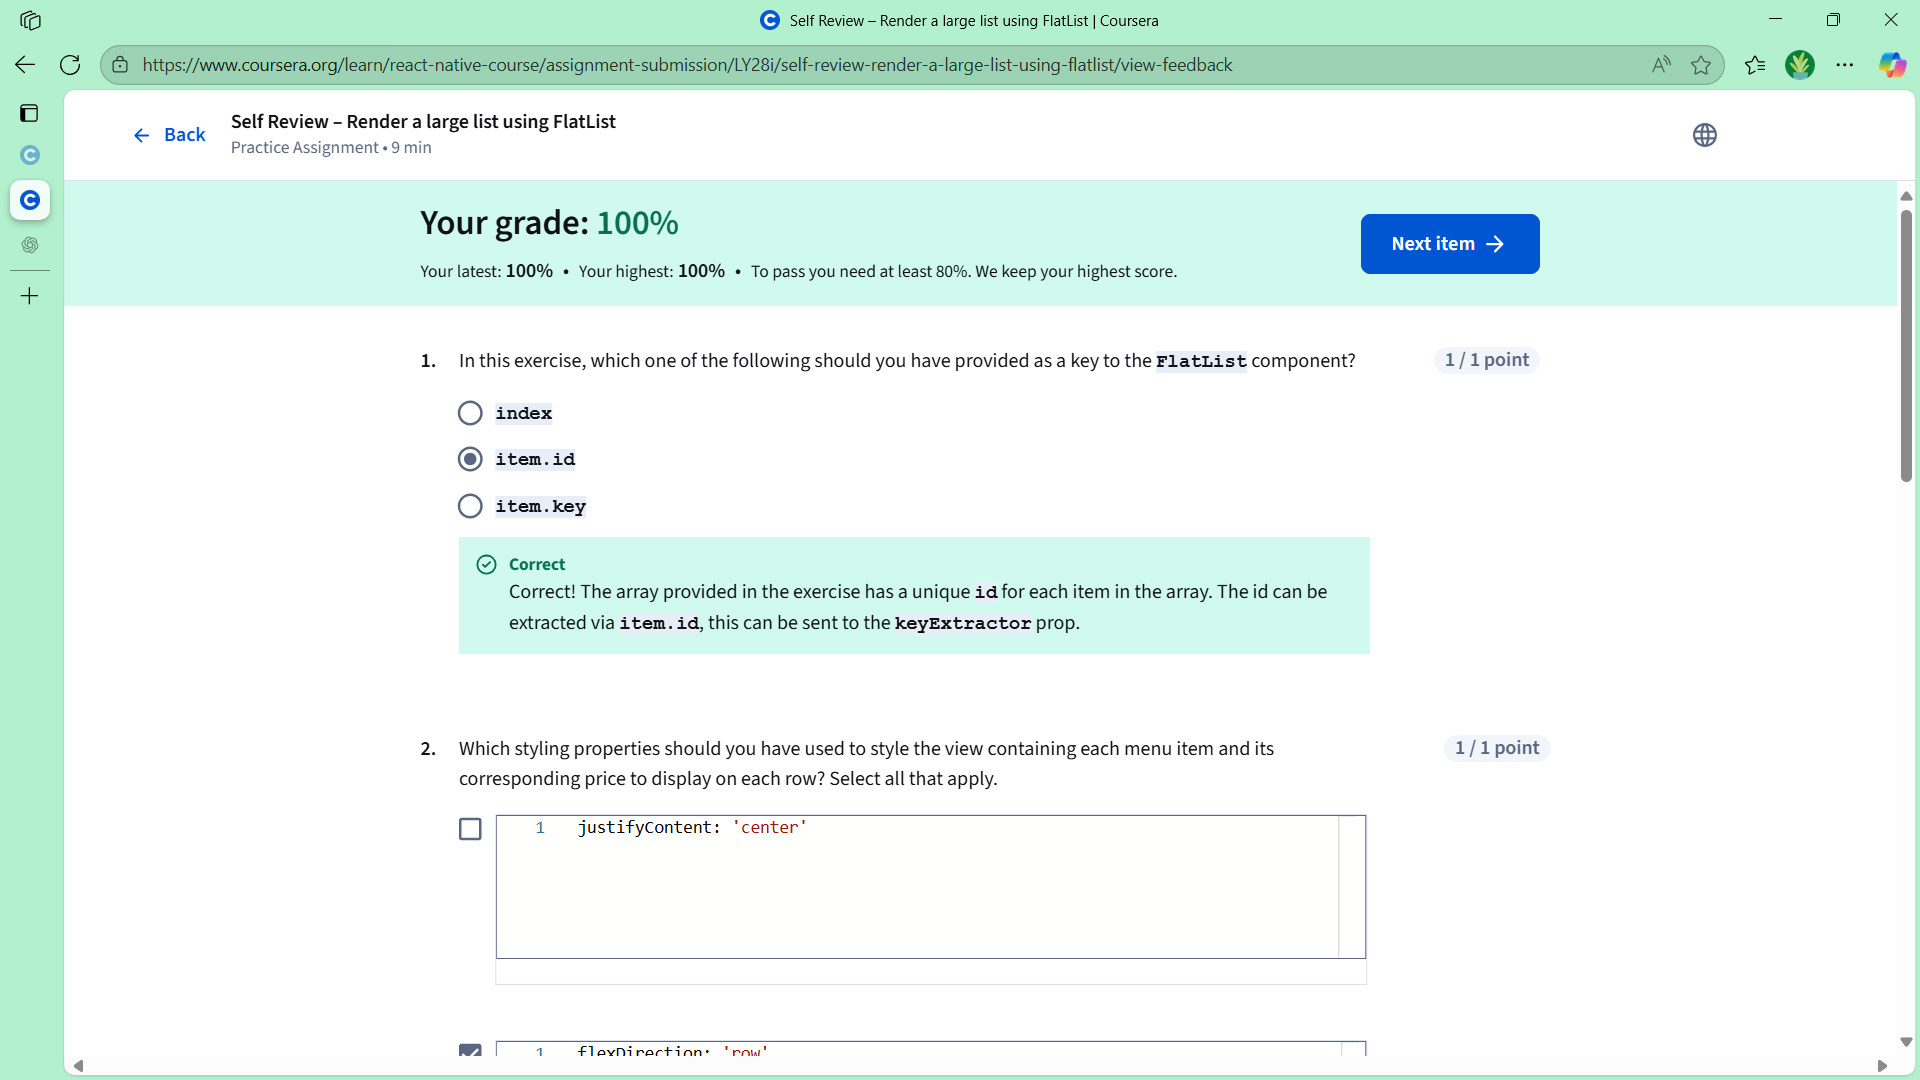
\includegraphics[width=0.5\linewidth]{images/sr-1.png}
    \caption{Self review: Render a large list using FlatList}
\end{figure}

\section{Video: FlatList Methods}
\subsection{keyExtractor}
\begin{itemize}
    \item Using \texttt{keyExtractor} for caching and as the react key to track item recording.
    \item Using at the same as using \texttt{map()} in react, we need to pass a key props.
\end{itemize}

\subsection{ItemSeperatorComponent}
\begin{itemize}
    \item Using: 
    \begin{lstlisting}[language=Java, numbers=none]
        const Seperator = () => <View style={menuItemsStyle.seperator} />

        <FlatList
            data={menuItemsToDisplay}
            keyExtractor={(item) => item.id}
            renderItem={renderItem}
            ItemSeparatorComponent={Seperator}
        />
    \end{lstlisting}
\end{itemize}

\subsection{ListHeaderComponent}
\begin{itemize}
    \item Using: 
    \begin{lstlisting}[language=Java, numbers=none]
        const Header = () => <Text style={menuItemsStyle.headerText}>View Menu</Text>

        <FlatList
            data={menuItemsToDisplay}
            keyExtractor={(item) => item.id}
            renderItem={renderItem}
            ItemSeparatorComponent={Seperator}
            ListHeaderComponent={Header}
        />
    \end{lstlisting}

    \item \textbf{Practice Question:} In your app, you have written a header component, and then rendered that component inside of \texttt{FlatList} and passed it to the \texttt{ListHeaderComponent} prop. When the user scrolls through the list in the app, this header will remain fixed in place. True or false?
    $\rightarrow$ False
\end{itemize}

\subsection{ListFooterComponent}
\begin{itemize}
    \item Using: 
    \begin{lstlisting}[language=Java, numbers=none]
        const Footer = () => <Text style={menuItemsStyle.footerText}>Footer</Text>

        <FlatList
            data={menuItemsToDisplay}
            keyExtractor={(item) => item.id}
            renderItem={renderItem}
            ItemSeparatorComponent={Seperator}
            ListHeaderComponent={Header}
            ListFooterComponent={Footer}
        />
    \end{lstlisting}
\end{itemize}

\section{Practice Assignment: Knowledge Check: Render large lists with FlatList}
\begin{figure}[H]
    \centering
    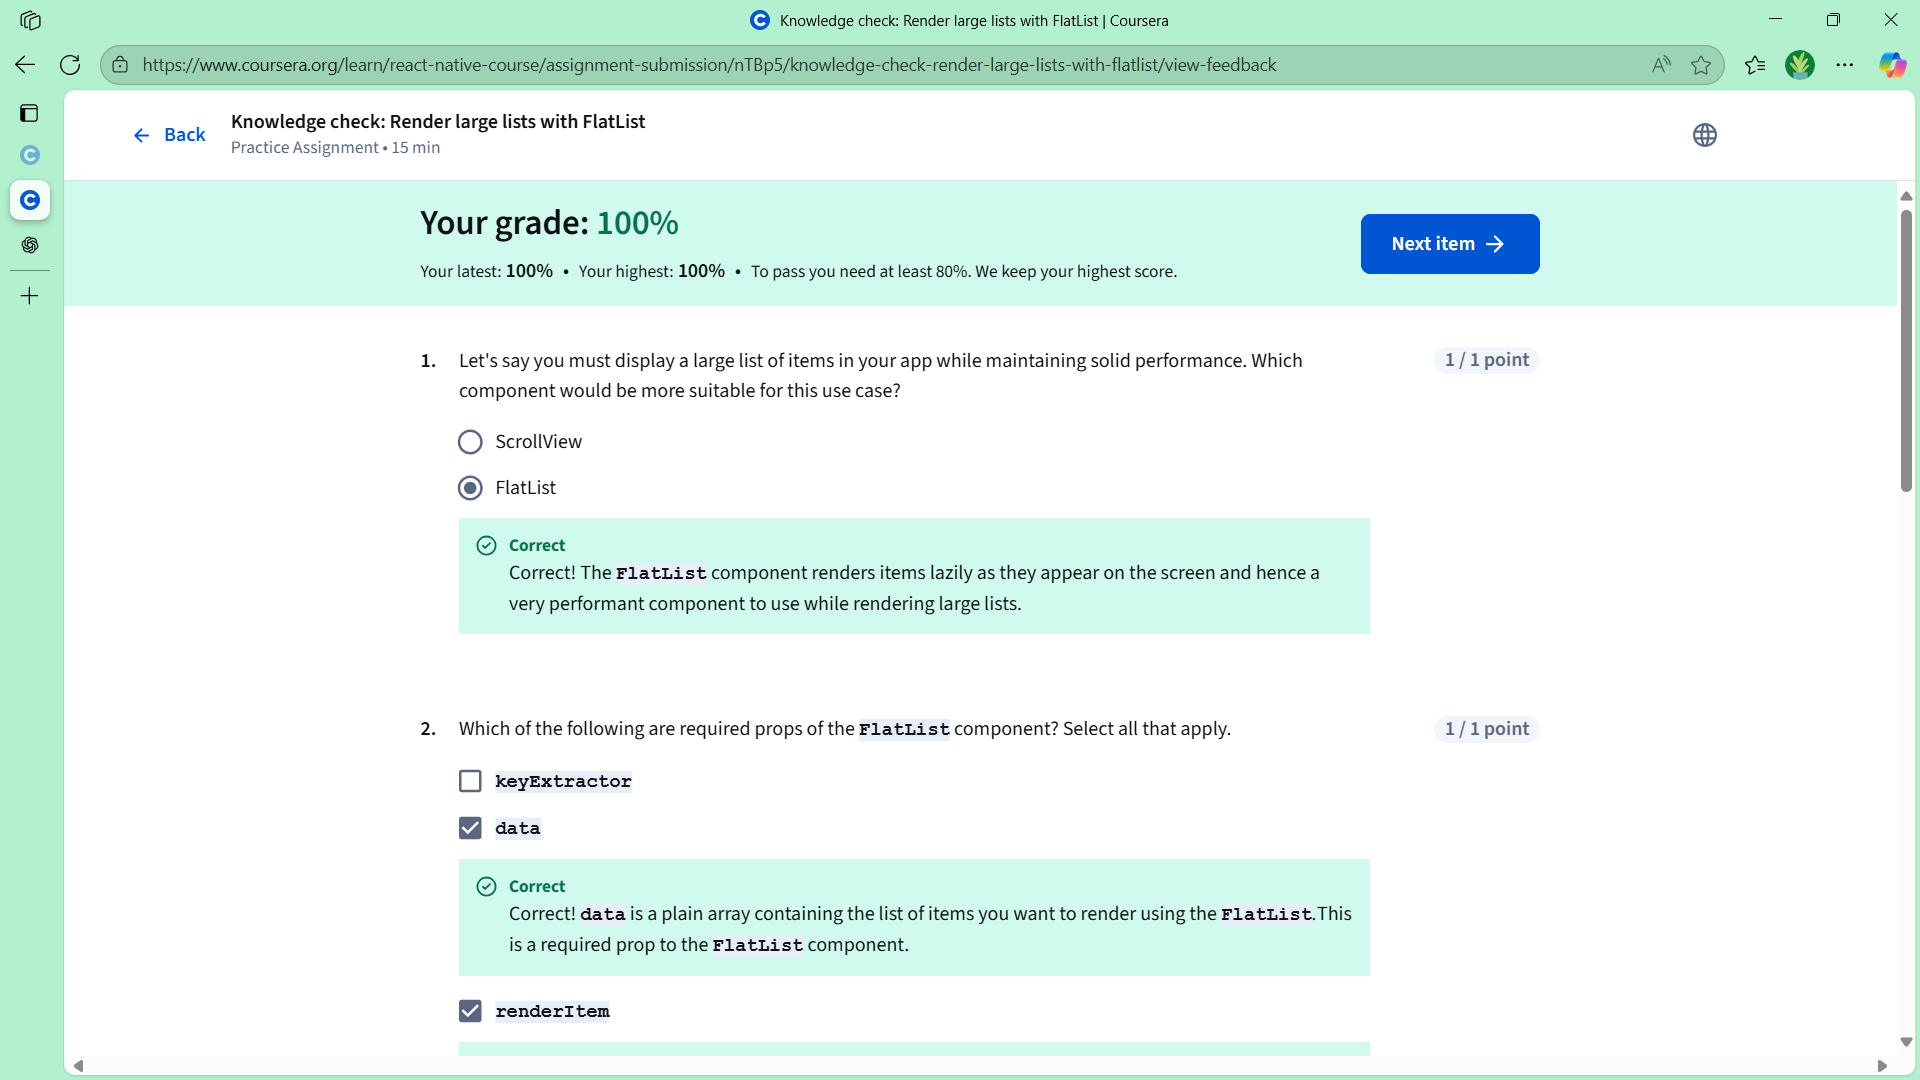
\includegraphics[width=0.5\linewidth]{images/kc-1.png}
    \caption{Knowledge Check: Render large lists with FlatList}
\end{figure}